% !TeX root = index.tex
\iffalse
This chapter presents the background physical or electrical theory
and on any analytical methods you will use to accomplish your goals.
If you have a research question, what is it?
Have you made any deductions from it that you are now testing?
What mathematical bases must be understood in order to interpret your results in Chapter 5?
Give the reader a solid understanding of the foundations here.
\fi

\iffalse
Figure \ref{fig:simple_blocks} represents simplified diagrams of RISC and OISC architectures. In RISC and CISC architecture, program data travels from program memory to the control block where instruction is decoded. Then control block further decides how data is directed in the datapath block which is described in section \ref{sec:datapath}. Such structure requires a complicated control block and additional data routing blocks. In order to increase the performance of one such processor you would need to add pipelining or multiple cores. Both methods have disadvantages: multicore processor requires software adjustments and each core doubles the control and datapath blocks, substantially increasing transistor count; pipelinig allows operation at higher frequencies however it brings design complications such as complicated hazard prevention logic and instruction lookup. RISC architecture in this project is mainly based on theory in \autocite{harris_harris_2013}. The simplicity of OISC architecture overcomes these disadvantages:

Pipelining can be done by individual blocks and programmibly waiting for results, this is represented in figure \ref{fig:oisc_simple} Adder and Multiply vertical blocks, multicore can be simulated by adding more data and instruction buses, hazards can be prevented with software and/or integrated into address registers.
\\ 
ALU and other processor components can be divided by adding different address registers. This allow utilisation of multiple components at the same time given that multiple data buses are used. This is represented in figure \ref{fig:oisc_simple} Arithmetic Unit horizontal blocks. Assuming 4 data and instructions buses are used, \textbf{AND} and \textbf{OR} blocks sources A and B can all be written during one cycle utilising both blocks at the same time.
\\
These 
\\
\fi

In this section differences in RISC and OISC are explained. It includes predictions and theory behind it. 

\subsection{RISC Processor}

\begin{figure*}[t!]
	\centering
	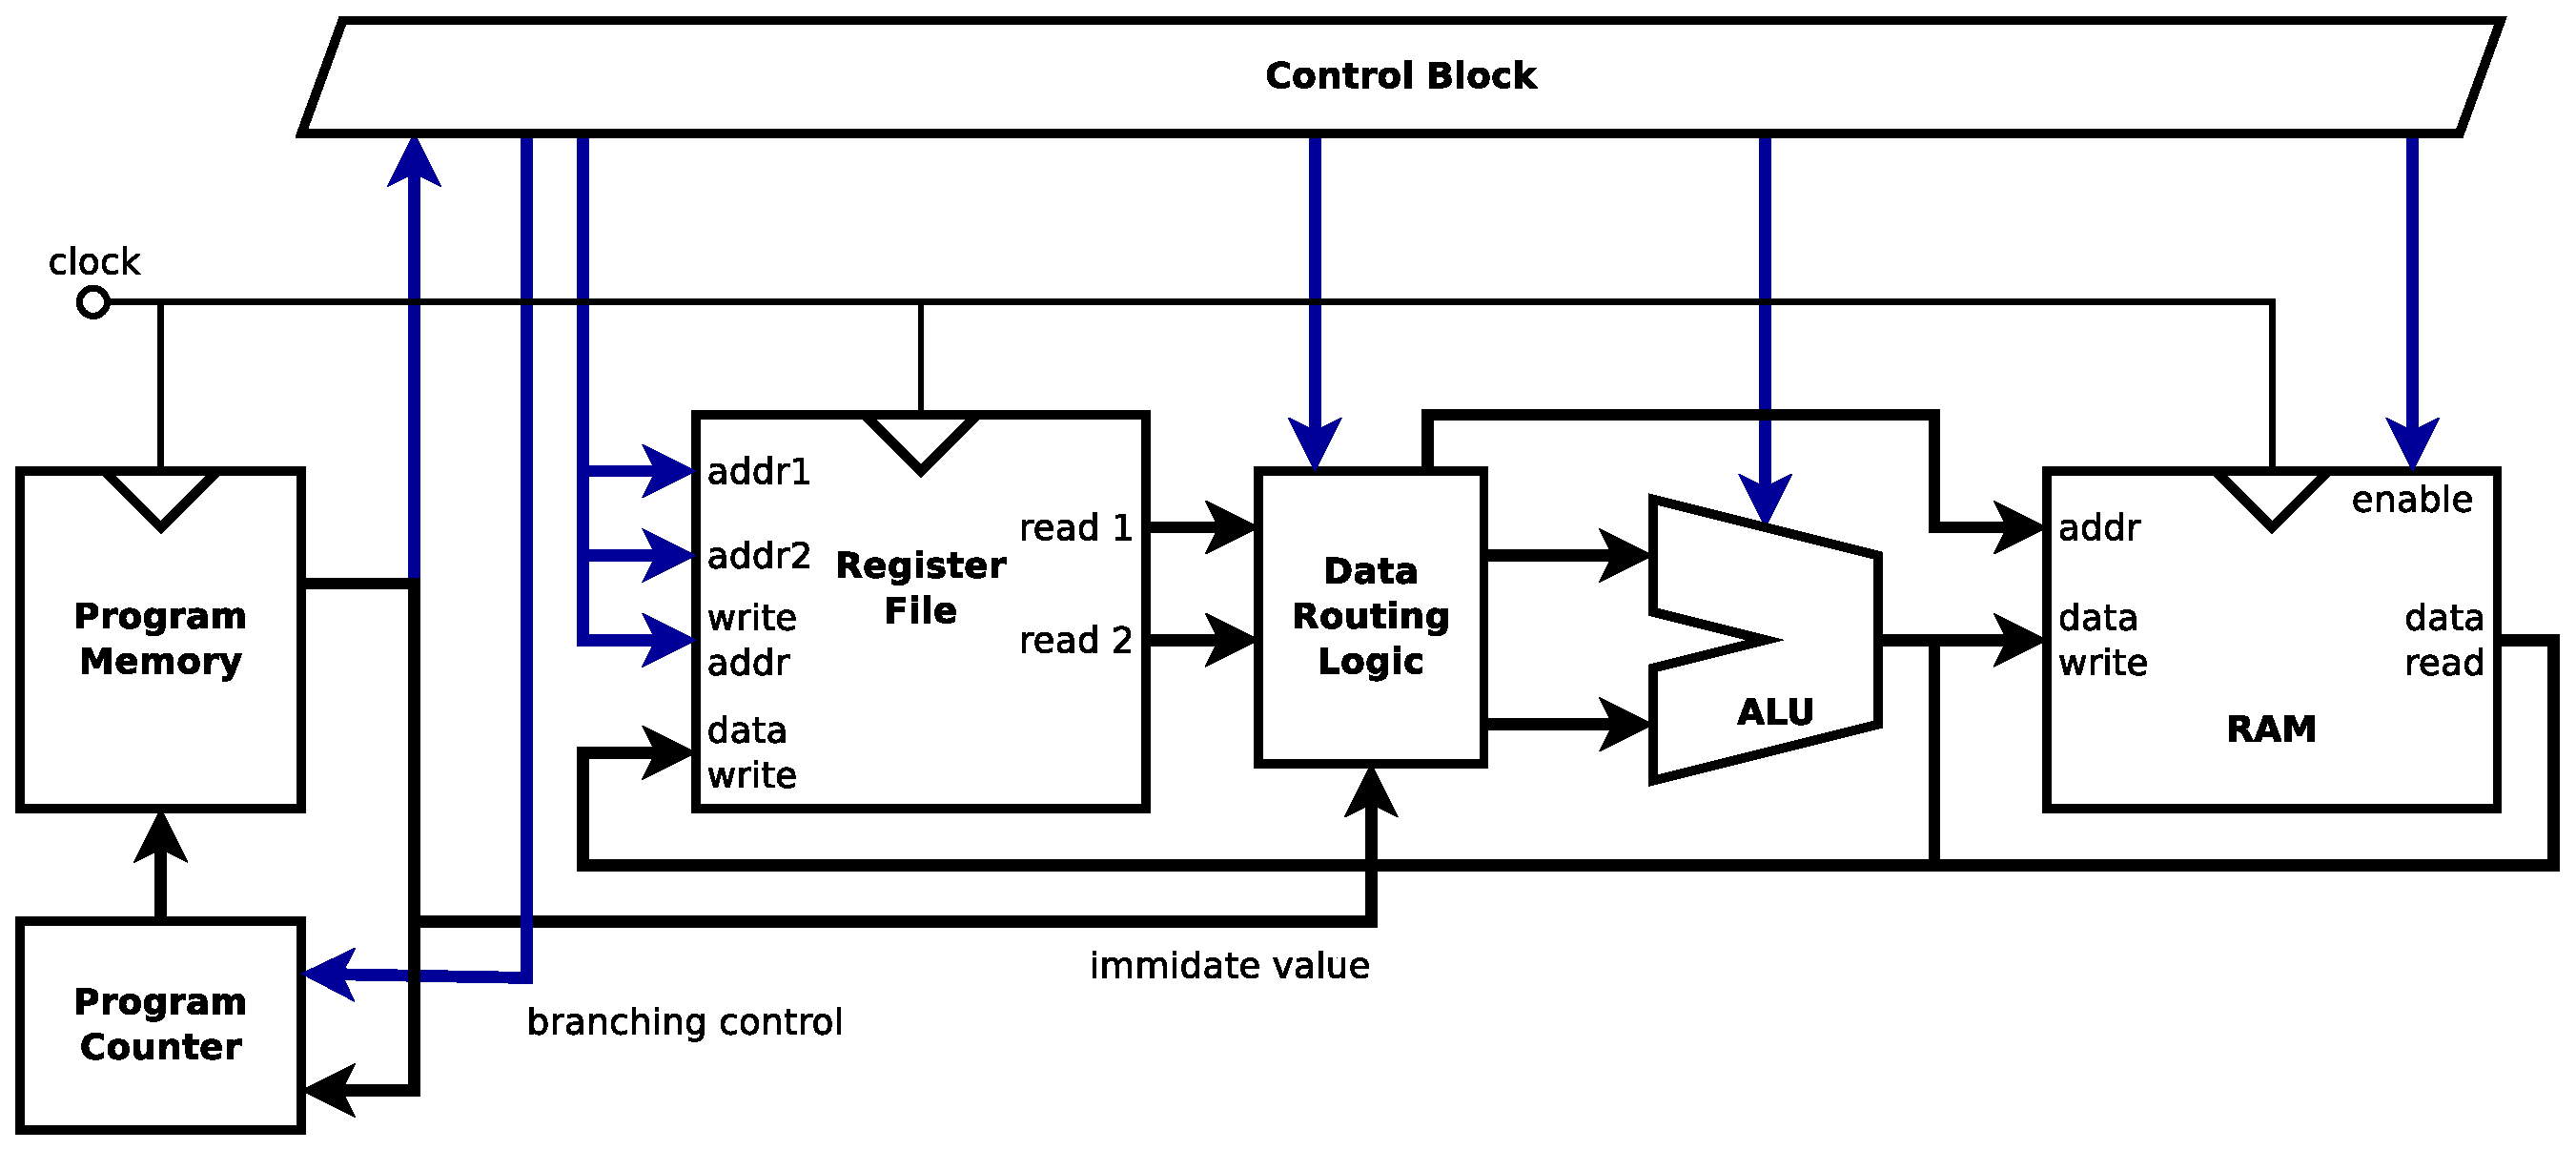
\includegraphics[width=\linewidth]{../resources/risc.eps}
	\caption{Abstract diagram of proposed RISC structure}
	\label{fig:risc_simple}
\end{figure*}

In this project, the proposed RISC is mainly based on the MIPS microarchitecture \autocite{harris_harris_2013}. Figure \ref{fig:risc_simple} represents a simplified diagram of a proposed RISC processor. In this architecture, program data travels from a program memory to the control block where the instruction is decoded. Then, the control block further decides how data is directed in the datapath block. Such structure requires a complicated control block and additional data routing blocks. Depending on the instruction, control block sets ALU, register file, memory operations and how data flows from one to other. Therefore, if none of the blocks are bypassed, data can flow though every single one of these blocks, creating a long chain of combinational logic and increasing the critical path. However, this enables great flexibility allowing multiple operations to be carried out during a single step, for example load value from register to memory, while address value is immediate offset by another register value using the ALU. In order to increase performance of such processor, pipelining or multiple cores may be used.

\subsubsection{Pipelining}
\begin{multline}\label{eq:tc}
	\begin{split}
	T_c =& t_{pcq} + t_{ROM} + t_{register} + \\
	 	 & t_{routing} + t_{ALU} + t_{RAM} + t_{setup}
	\end{split}
\end{multline}

Equation \ref{eq:tc} shows the maximum processor cycle period $T_c$ which depends on combinational logic delay of every logic block, flip-flop time of propagation from clock to output of synchronous sequential circuit $t_{pcq}$ and flip-flop setup time $t_{setup}$.

\begin{align}\label{eq:tcp}
	T_{cp} &= max \left( \begin{matrix}
	t_{pcq} + t_{ROM} + t_{setup},\\
	t_{pcq} + t_{register} + t_{setup},\\
	t_{pcq} + t_{ALU} + t_{setup},\\
	t_{pcq} + t_{RAM} + t_{setup}\\
	\end{matrix}\right)
\end{align}

Pipelinig separates each processor's datapath block with a flip-flop. This changes critical path therefore reducing cycle period. A pipelined processor cycle period $T_{cp}$ is represented in the equation \ref{eq:tcp}. Such modification could theoretically increase clock frequency by 2 or 3 times.

Pipelining, however, introduces other design complications. Instructions that depend on each other, for example an operation $R = A + B + C$ needs to be executed in two steps, $t = A + B$ and $R = t + C$. The second step depends upon previous step result. Therefore, additional logic is required to detect such dependencies and bypass datapath stages, or stall pipelining. Furthermore, branching would also require stalling; temporary saving datapath stage and restoring it if needed when branching is concluded; or further branch prediction logic. Such dependency and branching issue requires timing hazards prevention logic which increases processor complexity and required resources. 

\subsubsection{Multiple cores}

A multicore system is a solution to increase processor throughput by having multiple datapaths and control logic instances, each running separate instructions. Cores share other system resources such as RAM.

A multicore processor requires software adjustments as each processor's core would execute separate programs. Therefore, some synchronisation between them is needed. A single additional core would also double the control and datapath blocks, substantially increasing resource requirements too. In addition, programs most often cannot be perfectly divided into parallel tasks due to some result dependencies between each subtask. Therefore, doubling processor core count would not likely result in doubling the performance. 

\subsection{OISC Processor}

\begin{figure*}[t!]
	\centering
	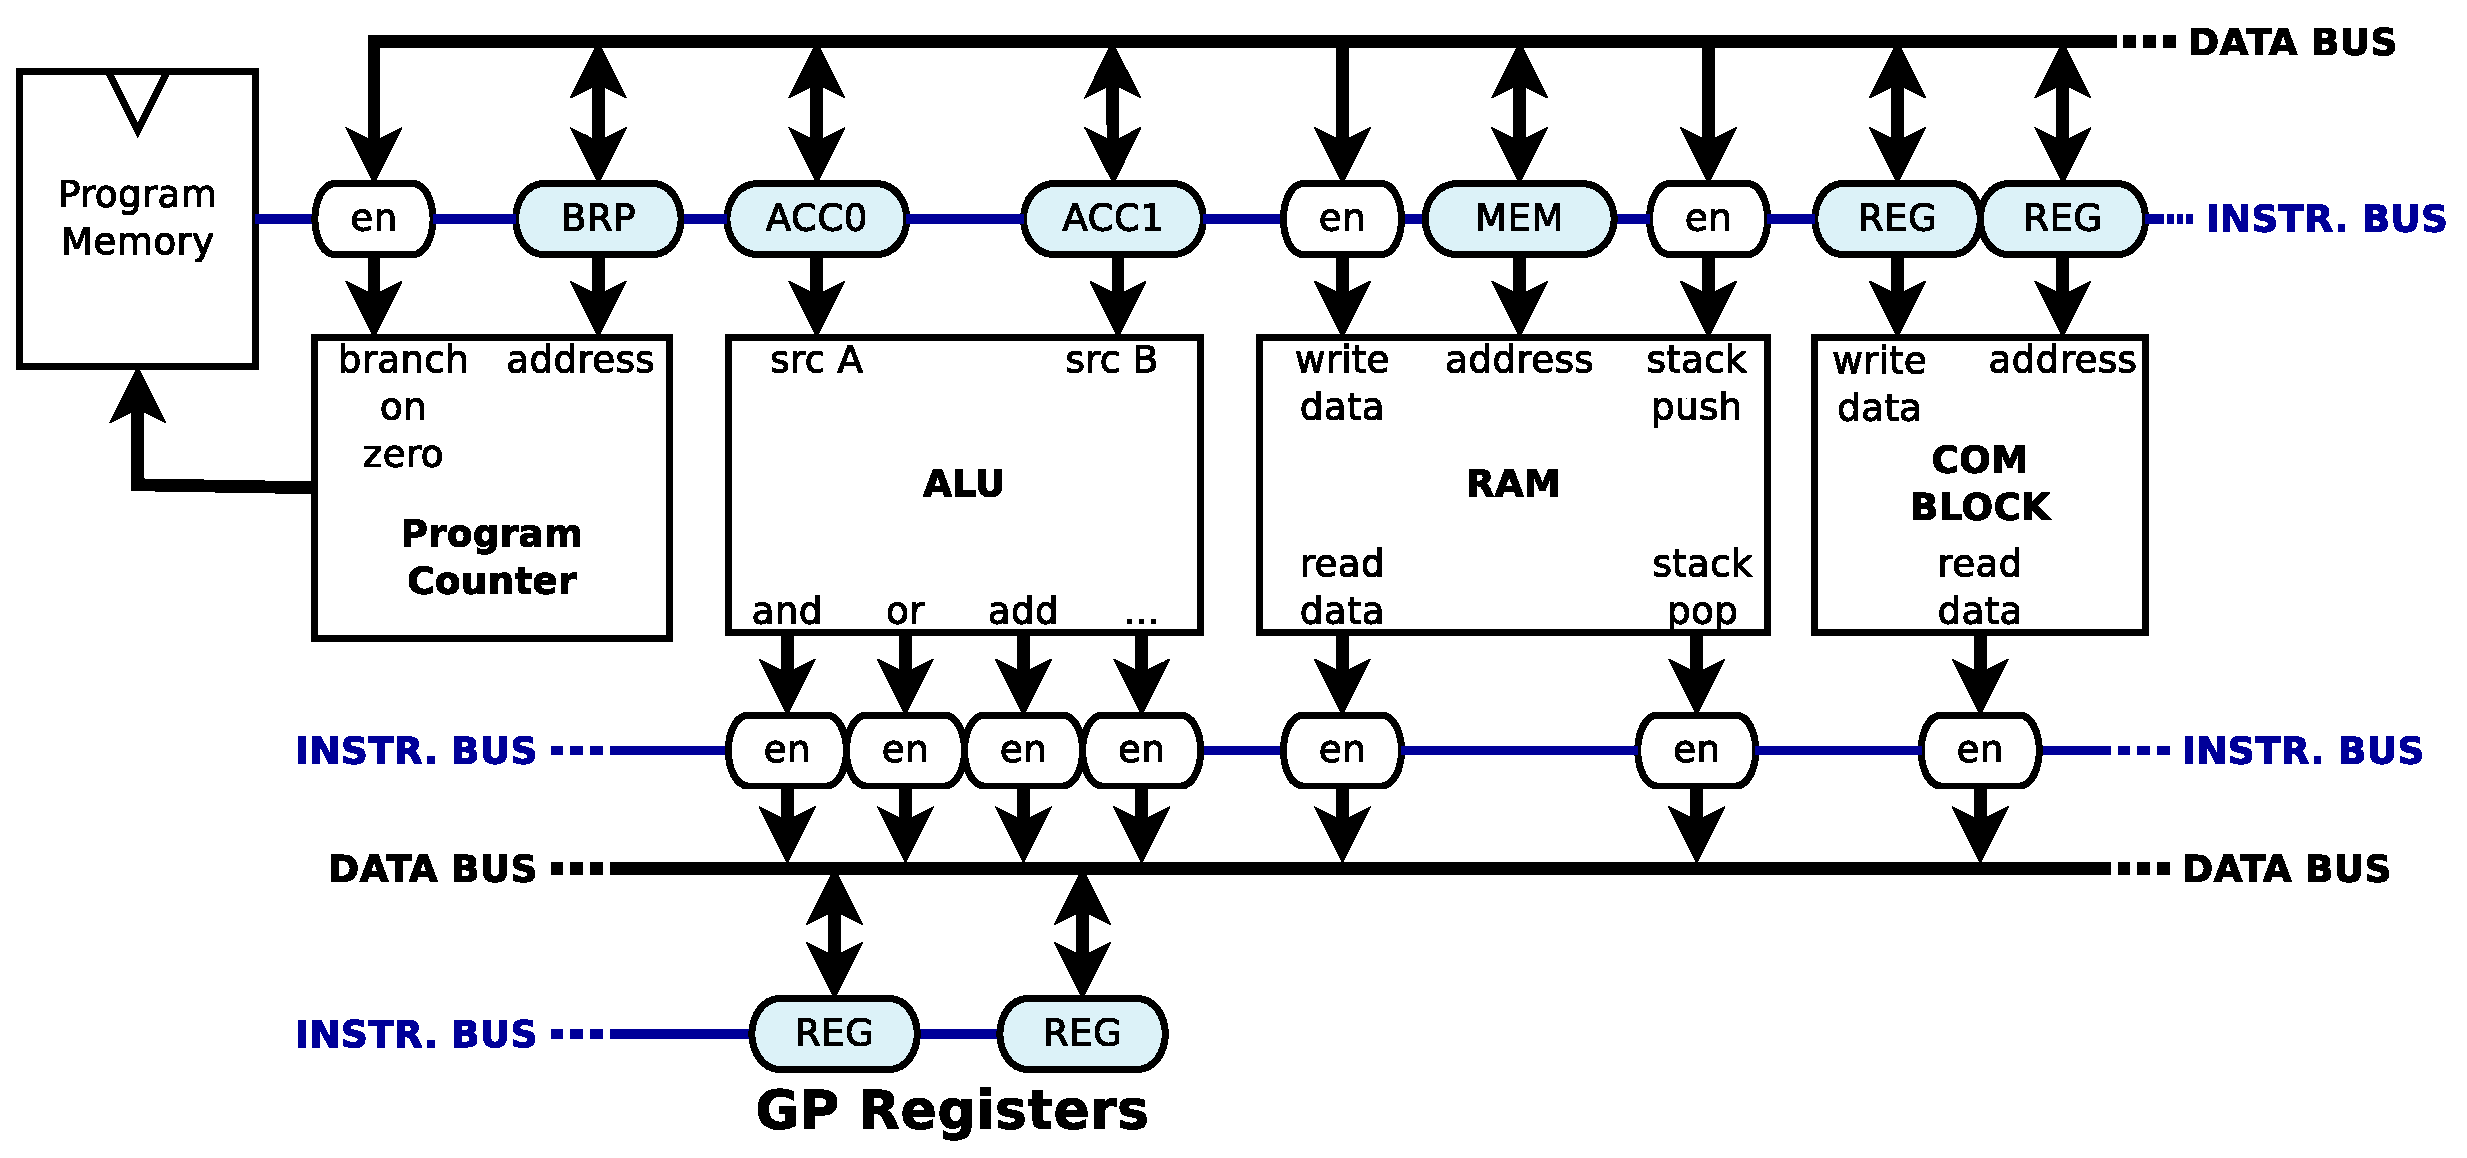
\includegraphics[width=\linewidth]{../resources/oisc.eps}
	\caption{Abstract diagram of proposed OISC structure}
	\label{fig:oisc_simple}
\end{figure*}

Figure \ref{fig:oisc_simple} represents simplified structure of an OISC MOVE architecture. In the simplest case, the processor has a pair of buses — data and instruction. An instruction bus has a source and destination address that connects two parts of processor via a data bus. This mechanism allows for the data to flow around processor. Computation is accomplished by setting accumulators at destination addresses and taking computed values from the source address. Other actions can be performed by destination node, for instance checking values for branching or sending data to memory. 

\subsubsection{OISC Pipelining}
The maximum cycle period of such processor microarchitecture can be found in Equation \ref{eq:oisc_tc}. 

\begin{multline}\label{eq:oisc_tc}
	\begin{split}
t_{CL} &= max \left( \begin{matrix}
t_{register},\\
t_{ALU},\\
t_{RAM}\end{matrix}\right)\\
&\\
T_{cp} &= max \left( \begin{matrix}
t_{en} + t_{buf},\\
t_{pcq1}\end{matrix}\right) +\\
&\qquad\qquad+ t_{pcq2} + t_{CL} + t_{setup}
	\end{split}
\end{multline}


Where $t_{en}$ is the period to check if instruction bus address match, $t_{buf}$ is period for source buffer to output value into the data bus, $t_{pcq2}$ is the propagation period for program memory, $t_{CL}$ represents the longest propagation period though a logic block, $t_{setup}$ is the setup time inside the logic block. $t_{pcq1}$ and $t_{pcq2}$ are clock to output delay for the sequential logic connecting source buffer and memory connecting instruction bus, respectively. 

\subsection{Predictions}

Comparing RISC and OISC, the maximum processor cycle period of OISC is almost equivalent to the pipelined RISC, with addition of enable, buffer and additional ROM delays: $max \left( t_{en} + t_{buf}, t_{pcq1}\right)$.

Furthermore, due to the nature of the processor no additional timing hazard prevention logic is needed, making this a much simpler design. OISC $t_{CL}$ pipelining can be also introduced to components that has high propagation delay. For instance, multiplication in an ALU could be pipelined into two stages. When setting ALU accumulators, software could be designed to retrieve multiplied result only after two cycles. This can further reduce required resources.

\subsubsection{Execution time}
OISC requires taking extra steps to perform basic functions. ALU, branch or memory operations need accumulator values to be set first to compute an output. A single data-instruction bus OISC therefore is expected to be slower executing the same task as RISC.

\subsubsection{Instruction Space}
RISC has compact instructions, as a single instruction can carry a small opcode, register addresses and optionality a multiple word immediate value. OISC has a bigger instruction overhead as it can only carry a source and destination address, meaning it can operate on only one register or immediate value in a single instruction. Therefore, it is expected the OISC will require more instruction space to perform the same function as RISC.

\subsubsection{Resources}
OISC does not have a control block which contains how data travels in the datapath. It also does not have multi-address register file and further routing logic within a datapath. This indicates that the OISC should require fewer logic elements to implement. This also should result in lower power consumption. 
%There are many papers looking into application specific TTAs. 